\documentclass[12pt]{article}

\usepackage[margin=1in]{geometry}

\usepackage{graphicx}
\graphicspath{ {paper_figures2/} }

\usepackage{amssymb,amsfonts,amsmath}
\DeclareMathOperator*{\argmin}{arg\,min}


\begin{document}

\section{Experimental Methods}

\subsection{Measuring developmental time during cellularization}

\begin{figure}[h!]
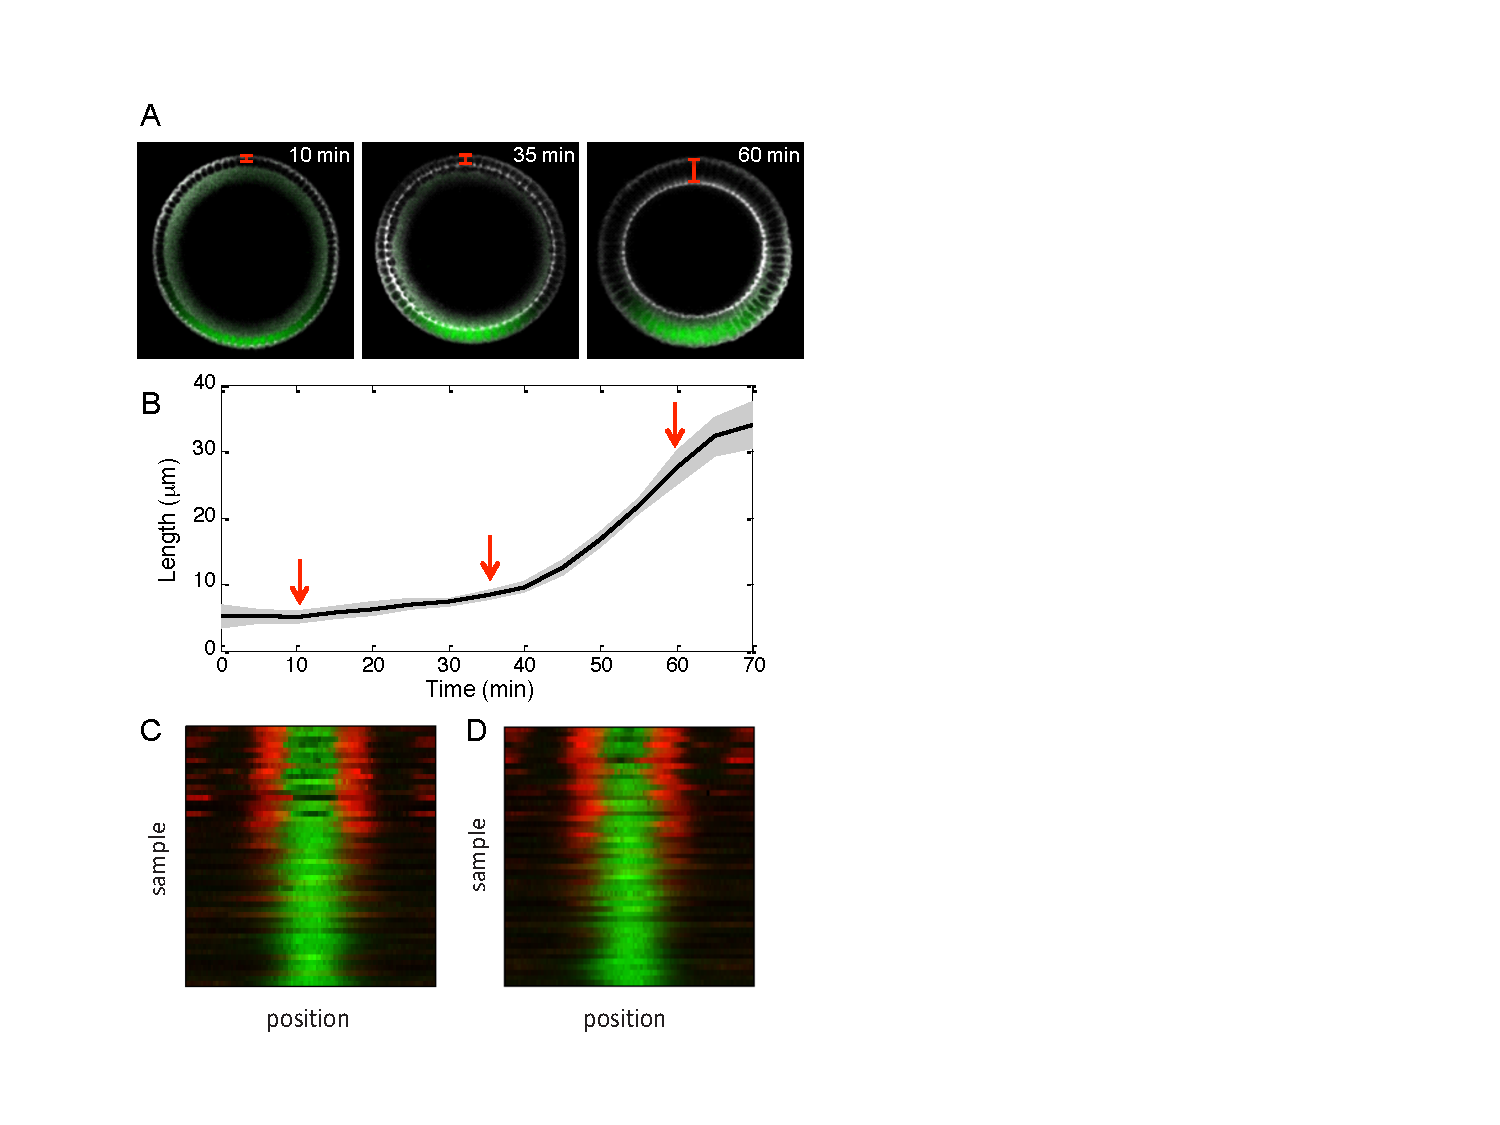
\includegraphics[width=8.4cm, trim=0cm 5.6cm 0cm 0cm, clip]{fig6}
\caption{{\it (A)} Images, stained for membranes (gray) and Dorsal (green) at different levels of development. {\it (B)} Membrane length as a function of time. The points corresponding to the images in {\it A} are indicated with arrows.}
\label{fig:membrane_compare}
\end{figure}

\section{PCA for gastrulating images}

\begin{figure}[h!]
\raisebox{5.2cm}{A}
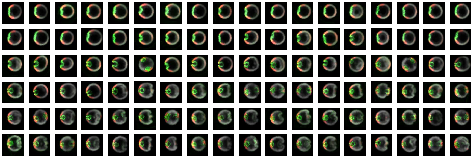
\includegraphics[width=16.8cm]{data2_PCA_ordered}

\raisebox{3.7cm}{B}
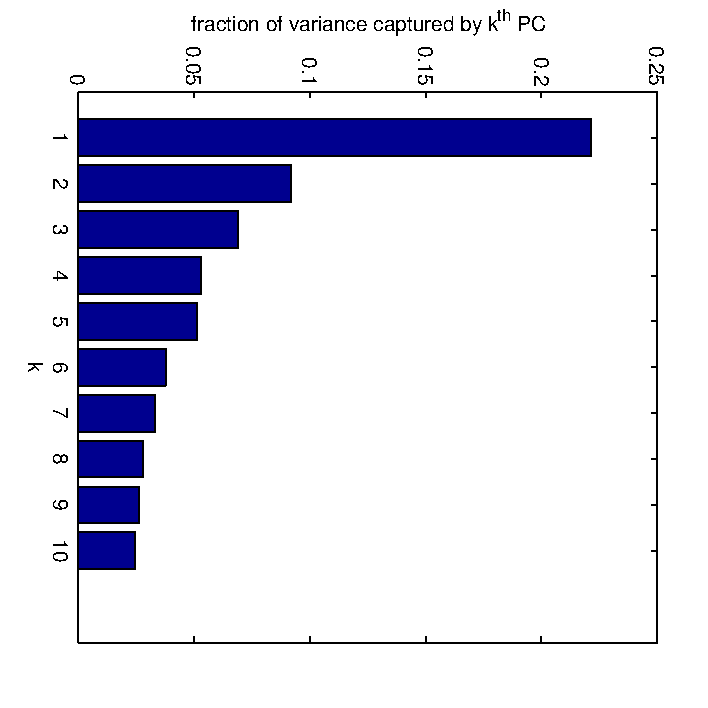
\includegraphics[width=8.4cm]{data2_PCA_variance}
\caption{{\it A} Images shown in Figure~4 of the paper, now ordered by the first PCA projection coefficient. Note that the ordering is not consistent with the developmental dynamics. {\it B} The eigenvalue spectrum from PCA. Note that subsequent components have a nonnegligible contribution on the data.}
\end{figure}

\section{Mathematical Algorithms}

\subsection{Angular synchronization \cite{singer2011angular}}

Let $ x_1, \dots, x_m$ denote the signals that we wish to align with respect to rotations;
each signal is a function defined on the unit circle (on the plane).
%
%Practically, it is discretized in a $n$-long vector (the local intensity at $n$ equidistant points around the circle);
%rotating the function by an angle $\theta$ then corresponds to cyclically shifting the elements of $x_i$ by $\frac{\theta_i}{2 \pi} n$ (rounded to the nearest integer to obtain a valid shift).
%
First assume that each signal $x_i$ is a {\it noisy} rotated copy of the underlying signal $x_{true}$
(which we are {\it not} given), such that
\begin{equation}
x_i = f(x_{true}, \theta_i) + \xi_i
\end{equation}
where the function $f(x_{true}, \theta_i)$ rotates the signal $x_{true}$ by $\theta_i$ radians, and $\xi_i$ is a (typically Gaussian) noise term.
%
Our goal is to recover $\theta_1, \dots, \theta_m$.
%
Up to noise,
\begin{equation} \label{eq:pairwise_rot}
x_i \approx f(x_j, \theta_i - \theta_j) ;
\end{equation}
note that \eqref{eq:pairwise_rot} does not require knowledge of $x_{true}$.
%
We can obtain an {\it estimate} of $\theta_i - \theta_j$ by computing the rotation that optimally aligns $x_j$ to $x_i$,
i.e., %$\theta_{ij} \approx \theta_i - \theta_j$, where
%
\begin{equation} \label{eq:opt_angle}
\theta_i - \theta_j \approx \theta_{ij} = \argmin_{\theta} \|x_i - f(x_j, \theta)\|^2.
\end{equation}
%
Practically, the signals are discretized in a $n$-long vector (the local intensity at $n$ equidistant points around the circle);
rotating the function by an angle $\theta$ then corresponds to cyclically shifting the elements of $x_i$
by $\frac{\theta_i}{2 \pi} n$ (rounded to the nearest integer to obtain a valid shift).
%
For the one-dimensional discretized profiles shown in Figure~\ref{fig:1d_demo}, we exhaustively search over all $n=100$ possible shifts of the signals to compute the optimal angles in \eqref{eq:opt_angle}.
%
Alternatively, for continuous signals, an optimization algorithm
can be used \cite{ahuja2007template}.

Rather than work with the angles $\theta_{ij}$ directly, it is more convenient to consider the	 rotation matrices,
\begin{equation} \label{eq:R_theta}
R(\theta_{ij}) = \begin{bmatrix}
\cos(\theta_{ij}) & -\sin(\theta_{ij}) \\
\sin(\theta_{ij}) & \cos(\theta_{ij})
\end{bmatrix},
\end{equation}
which we can think of as operating on the points of the unit circle (on the plane) on which our signal is defined.
%
Successive rotations correspond to multiplication of the corresponding rotation matrices: $R(\alpha_1 + \alpha_2) = R(\alpha_1) R(\alpha_2)$.
%
Due to the orthogonality of rotation matrices, $R(-\alpha) = R(\alpha)^T$.

Let $d$ denote the dimension of the rotation matrices we are considering (for our example of planar rotations, $R(\theta_{ij}) \in \mathbb{R}^{2 \times 2}$ and $d=2$; we write our procedure for general $d$ because we will later consider three-dimensional rotations).
%
We construct the matrix $H \in \mathbb{R}^{md \times md}$, where $H$ is an $m \times m$ matrix of $d \times d$ blocks, with the $i,j^{th}$ block of $H$, $H_{ij}$, defined as
\begin{equation} \label{eq:H_to_R}
H_{ij} = R(\theta_{ij}).
\end{equation}
%
%
Under our assumption that $\theta_{ij} \approx \theta_i - \theta_j$, $H_{ij} \approx R(\theta_i) R(\theta_j)^T$
%\begin{equation}
%H_{ij} = R(\theta_{ij}) \approx R(\theta_i - \theta_j) = R(\theta_i) R(-\theta_j) = R(\theta_i) R(\theta_j)^T,
%\end{equation}
 and
\begin{equation} \label{eq:H_low_rank}
	H \approx
	\begin{bmatrix}
	R(\theta_1) \\
	R(\theta_2) \\
	\vdots \\
	R(\theta_m)
	\end{bmatrix}
	\begin{bmatrix}
	R(\theta_1)^T R(\theta_2)^T \dots R(\theta_m)^T
	\end{bmatrix}.
\end{equation}
%
It follows directly from \eqref{eq:H_low_rank} that the top block eigenvector of $H$ contains our best estimates of $R(\theta_1), R(\theta_2), \dots, R(\theta_m)$.
%
Let $\phi_1, \phi_2, \dots, \phi_{md}$ denote the eigenvectors of $H$, ordered such that $|\lambda_1| \ge |\lambda_2| \ge \dots \ge |\lambda_{md}|$, where $\lambda_i$ is the eigenvalue corresponding to $\phi_i$.
%
Then,
\begin{equation}
\hat{R} =
\begin{bmatrix}
\hat{R}_1 \\
\hat{R}_2 \\
\vdots \\
\hat{R}_m
\end{bmatrix} =
\begin{bmatrix}
| & | & & | \\
\phi_1 & \phi_2 & \dots & \phi_d \\
| & | & & |
\end{bmatrix},
\end{equation}
where $\hat{R}_i \in \mathbb{R}^{d \times d}$ is (nearly) the estimate for $R(\theta_i)$.
%
To obtain our estimate of $R(\theta_i$), denoted $R_{i, est}$, we project $\hat{R}_i$ onto the closest orthogonal matrix, 
\begin{equation} \label{eq:R_est}
R_{i, est} = U_i V_i^T,
\end{equation}
where $U_i$ and $V_i$ are the left and right singular vectors, respectively, of $\hat{R}_i$.
%
We adjust the sign of $\phi_1$ so that $det(R_{i, est}) = +1$, ensuring proper rotations.
%
We estimate $\theta_{i}$ by inverting \eqref{eq:R_theta}, and register the signals by rotating signal $i$ by $-\theta_i$.
%
We note that, in our actual computations, the pairwise rotations $\theta_{ij}$ are computed in a discrete setting, then the overall
synchronization is performed in the continuum context to obtain $\theta_i$, and the results are rounded to give the closest
discrete shift.
%
Details of registering two-dimensional images using synchronization are given in the {\it SI Appendix}. 

%Furthermore, this formulation also considers {\it higher-order} consistency information.
%
%For example, given our pairwise estimates $R_{ij}$, we know that relationships of the form
%\begin{equation} \label{eq:triplet_consistency}
%R(\theta_{ik}) R(\theta_{kj}) \approx R(\theta_i) R(\theta_k)^T R(\theta_k) R(\theta_j)^T = R(\theta_i) R(\theta_j)^T
%\end{equation}
%should also hold.
%
%Note that
%\begin{equation}
%(H^2)_{ij} = \sum_k R(\theta_{ik}) R(\theta_{kj});
%\end{equation}
%therefore, {\it all} infomation of the form in \eqref{eq:triplet_consistency} is contained in the matrix $H^2$.
%
%Because $H$ and $H^2$ have the same eigenvectors, our problem formulation accounts for not only pairwise alignment information, but also these higher-order considerations.

\subsection{Diffusion maps \cite{coifman2005geometric}}

Given $m$ data points $x_1, \dots, x_m$ (typically vectors in a high-dimensional space), we want to find a coordinate transformation $y(x)$ that preserves local information: points that are close in the original space should also be close in the coordinate $y$.
%
The first step is to construct the matrix $W \in \mathbb{R}^{m \times m}$, where $W_{ij}$ is large if points $x_i$ and $x_j$ are ``close.''
%
We use a diffusion kernel,
\begin{equation} \label{eq:dmaps_W}
W_{ij} = \exp \left( -\frac{d^2(x_i, x_j)}{\epsilon^2} \right)
%W_{ij} = e^{ -\frac{d^2(x_i, x_j)}{\epsilon^2}}
\end{equation}
where $d(x_i, x_j)$ is the pairwise distance between $x_i$ and $x_j$ (often the Euclidean distance), and $\epsilon$ is a characteristic scale.
%
Points less than $\epsilon$ apart are thus considered ``close'' and points farther than $\epsilon$ apart are considered ``far away''.
%
$\epsilon$ can be chosen using several techniques (see, for example \cite{coifman2008graph}); here, we take $\epsilon$ to be the median of the pairwise distances between data points.

To find this coordinate $y$, we want solve the following optimization problem \cite{Belkin2003}
\begin{equation} \label{eq:dmaps_opt_problem}
\argmin_{y} \sum_{ij} W_{ij} (y(x_i) - y(x_j))^2.
\end{equation}
%
We first compute the diagonal matrix $D$, where $D_{ii} = \sum_{j=1}^{m} W_{ij}$, and the matrix $A$, where
\begin{equation} \label{eq:dmaps_A}
A = D^{-1} W.
\end{equation}
%
We calculate the eigenvectors $\phi_1, \phi_2, \dots, \phi_m$, ordered such that $|\lambda_1| \ge |\lambda_2| \ge \dots \ge |\lambda_m|$.
%
%Because the matrix $A$ is similar to the symmetric matrix $D^{-1/2} W D^{-1/2}$, $A$ is guaranteed to have real eigenvalues and real, orthogonal eigenvectors.
%
Because the matrix $A$ is row-stochastic, $\lambda_1=1$ and $\phi_1$ is a constant vector; this is a trivial solution to \eqref{eq:dmaps_opt_problem}.
%
%In general, the next few eigenvectors $\phi_2, \dots, \phi_m$ give ``meaningful'' embedding coordinates for the data, such that $\phi_j(i)$ gives the $j^{th}$ embedding coordinate of the $i^{th}$ data point.
%
The next eigenvector, $\phi_2$, is the (non-trivial) solution to \eqref{eq:dmaps_opt_problem}, so that $\phi_2(j)$, the $j^{th}$ entry of $\phi_2$, gives the ``new" coordinate for data point $x_j$ (i.e., $\phi_2(j) = y(x_j)$).
%
In our application, we have assumed that this single direction of variability, parameterized by $\phi_2$, is one-to-one with time.
%
Ordering the data by $\phi_2(j)$ will then, effectively, order them in time.
%
The procedure generalizes when the data lie on higher-dimensional manifolds (not just curves) in data space.

\subsection{Vector diffusion maps\cite{singer2012vector}}

In vector diffusion maps, given data points $x_1, \dots, x_m$, one first constructs the matrix $S \in \mathbb{R}^{md \times md}$, with the $i,j^{th}$ block of $S$, $S_{ij}$, defined as
\begin{equation} \label{eq:vdm_S}
	S_{ij} = A_{ij} H_{ij}
\end{equation}
%
where $A_{ij} \in \mathbb{R}$ (defined in \eqref{eq:dmaps_A}) pertains to the diffusion kernel between data points, and $H_{ij} \in \mathbb{R}^{d \times d}$ (defined in \eqref{eq:H_to_R}) pertains to the pairwise alignment between data points.
%
It is important to note that distance $d(x_i, x_j)$ used in the diffusion kernel in \eqref{eq:dmaps_W} is the distance between data points {\it after} after pairwise alignment, i.e., the minimum distance between all possible shifts of the two data points (which is obtained in \eqref{eq:opt_pairwise}).
%
In the language of symmetry groups, this distance is a metric between the orbits induced by the symmetry group.

One then computes the eigenvalues $\lambda_1, \lambda_2, \dots, \lambda_{md}$ and eigenvectors $\phi_1, \phi_2, \dots, \phi_{md}$ of $S$, ordered such that $|\lambda_1| \ge |\lambda_2| \ge \dots \ge |\lambda_{md}|$.
%
These eigenvectors contain information about {\it both} the optimal rotations (the ``synchronization" component) and the
variation of the data {\it after} the spatial symmetries have been factored out (in our case, their temporal variation).
%
Assuming that the data (after symmetries have been factored out) are relatively closely clustered, it is reasonable
to expect, as in angular synchronization, that the top (block) eigenvector of $S$ contains approximations of the optimal rotations,
which can be computed in the same way from \eqref{eq:R_est}.
%
We then expect subsequent eigenvectors to contain information about the main direction(s) of data variability modulo the geometric symmetries.
%%%
%%% somewhere we need to talk about compact groups
%%% discussion might be a good place because SCALING is obviously important and
%%% it is not compact......
%%%
%However, the eigenvectors now also contain information about the embedding coordinates for our images.
%
In general, the embedding coordinates will be given by
\begin{equation}
\psi_{k,l} (i) = \langle \phi_k(i), \phi_l(i) \rangle
\end{equation}
where $\phi_k(i) \in \mathbb{R}^d$ denotes the $i^{th}$ block of $\phi_k$.
%
If we assume that our data mainly vary along a one-dimensional manifold, and that the rotations and the dynamics are uncoupled and therefore separable, one expects the embedding coordinate for our data %(i.e., the analog of $\phi_2$ from the diffusion maps case)
to be  $\psi_{1,d+1}$.
%
Our example is, by physical considerations, a separable one, and so sorting our data by $\psi_{1,d+1}$ will order our data in time.
%
If no separability claims can be made, a second diffusion map step, using $\psi_{k,l}$ as the coordinates, may uncover a
useful parameterization of the data manifold modulo symmetries.




\section{Registering images with respect to translations and rotations} \label{subsec:trans_rot_register}

Using angular synchronization or vector diffusion maps to register images with respect to rotations {\it and translations} requires some additional effort.
%
%We are not only interested in registering the one-dimensional concentration profiles with respect to rotational symmetries, but we would also like to register the two-dimensional images shown in Figure \ref{fig:fluorescent_images} with respect to rotations {\it and} translations.
%
%We first compute the translations and rotations to optimally align each pair of data points.
%
The first step (similar to the case of only rotations) is to compute the optimal alignments between pairs of images.
%
Practically, we have square images discretized as pixels (rather than continuous functions on the plane).
%
For each image pair $I_i$ and $I_j$ we compute
\begin{equation}\label{eq:opt_pairwise}
(\theta_{ij}, dx_{ij}, dy_{ij}) = \argmin_{
\begin{matrix}
\theta \in [0, 2\pi) \\
dx, dy \in [-\Delta, \Delta]\\
%dy \in [-\Delta, \Delta]
\end{matrix}
} \|g(I_j, \theta, dx, dy) - I_i \|^2.
\end{equation}
where $g(I_j, \theta, dx, dy)$ is image $I_j$ rotated around the center of the square by $\theta$ radians, then translated by $dx$ pixel widths in the $x$ direction, and finally translated by $dy$ pixel widths in the $y$ direction.
%
The norm, $\| \cdot \|$, is the Euclidean norm between the pixel intensities for both the red and green channels.
%
The domain of the image (a square) is not invariant to our rotations and translations; however, the pixels near the border of the square have zero intensity, and so the norm can be meaningfully computed as long as the main image does not ``move out of'' the original square.
%
%The norm \eqref{eq:opt_pairwise} involve an integral over the square, which is not left invariant by our rotations and
%translations; noting however that the pixels close to the border of the square have zero intensity allows a meaningful
%computation of this norm as long as the ``main feature" (the embryo) does not move out of the original square (no ``corner effects").
%
This also justifies the $\Delta$ limits in \eqref{eq:opt_pairwise}: $\Delta$ is chosen such that the main image is not split or separated when translating (we take $\Delta=10$, which corresponds to a 10\% shift in the image). 
%; it does not make sense to shift the images so much that the embryo would ``move out" of the original square.
%
Image rotation is performed with the \texttt{imrotate} function in Matlab, using nearest neighbor interpolation to estimate the pixel intensities after rotation.
%, since there is no direct mapping of the pixels of the unrotated image to the pixels of the rotated image.
%
The missing pixels in the corners of the rotated image are taken to have zero intensity.
%
The translations are implemented by shifting the pixels;
we only consider shifts that correspond to an integer number of pixels to remove the need for interpolation when doing the translations.
%
The solution to \eqref{eq:opt_pairwise} is not easily computed, as the objective function will most likely be nonconvex.
%
Therefore, instead of using an optimization procedure, we discretize the search space and exhaustively search to find the solution.
%
Our discrete translation steps are $\Delta/5$, and our discrete rotations steps are $\pi/10$. 
%
%We discritize the search space of rotations into 20 possible rotations %($d\theta  \in \{0, \pi/10, \pi/5, \dots, 9 \pi/5, 19\pi/10 \}$),
%and 11 possible translations in both . %($dx, dy \in \{-20, -16, -12, \dots, 12, 16, 20 \}$).
%
%We check all possible combinations for the rotation and translations that best align $I_j$ to $I_i$.
%
Although computationally demanding, this ``embarrassingly parallelizable" direct enumeration approach is not prohibitive here.
%
%Although this can be somewhat time intensive, it is not prohibitive for the data sets we consider, and can be trivially parallelized if necessary.
%
%The solution will not be the exact solution to \eqref{eq:opt_pairwise}, but it will (most likely) be a close approximation.
%
%Since our techniques are robust to noise, close approximations will be sufficient to obtain accurate results.

%As discussed above, for angular synchronization, the underlying symmetry group needs to have a real and orthogonal matrix representation.
%
%We therefore convert $ISO(2)$, the group of two-dimensional translations and rotations, to $SO(3)$, the group of three-dimensional rotations.
%

The synchronization formulation requires that the matrices used to represent the symmetry group be orthogonal \cite{singer2013spectral}.  
%(for \eqref{eq:H_low_rank} to be satisfied).
%
However, the typical matrix representation for $ISO(2)$, the group of two-dimensional translations and rotations, does not satisfy this property.
%
Instead, we {\it approximately} represent rotations and translations in two dimensions using {\it three-dimensional rotation matrices}, by projecting the (two-dimensional) image onto a portion of the surface of a (three-dimensional) sphere \cite{singer2011angular}.
%
Rotation of the image corresponds to rotation around one principal axis in three dimensions, while translation of the image corresponds (approximately) to rotations around the other two principal axes. %(Clearly, not all translations can be described this way, as translations can range from $-\infty$ to $+ \infty$, and rotations are only from $0$ to $2 \pi$. However, the images we will be considering are already mostly centered, and so we are only interested in small translations that are well within the $[0, 2\pi)$ range.)
%
%These rotation matrices are (by definition) orthogonal, and successive applications of various translations and rotations can be described via multiplication of the corresponding rotation matrices in $SO(3)$.



To convert the optimal two-dimensional translation and rotation to corresponding (continuous) three-dimensional rotations,
we first compute the Euler angles $\alpha_{ij}$, $\beta_{ij}$, and $\gamma_{ij}$,
\begin{equation} \label{eq:angle_relations}
%\begin{aligned}
%	\alpha_{ij} &= \theta_{ij} \\
%	\beta_{ij} &= \frac{dx_{ij}}{n} \times \eta_{proj} \\
%	\gamma_{ij} &= \frac{dy_{ij}}{n} \times \eta_{proj} \\
%\end{aligned}
	\alpha_{ij} = \theta_{ij}, \; \; \;
	\beta_{ij} = \frac{dx_{ij}}{n} \times \eta_{proj}, \; \; \;
	\gamma_{ij} = \frac{dy_{ij}}{n} \times \eta_{proj}
\end{equation}
where $\eta_{proj}$ is the angular portion of the sphere onto which we choose to project the image.
%
We take $\eta_{proj} =  \pi/8$, so the image lies on a $\pi/8 \times \pi/8$ radians portion of the unit sphere;
this portion of the sphere is small enough so that curvature effects are not prominent in the image.
%
We write rotations around the three principal axes, $R^x(\alpha)$, $R^y(\beta)$, and $R^z(\gamma)$, in terms of the three Euler angles
%\small
\begin{equation}
\begin{aligned}
	R^x(\alpha) &= \begin{bmatrix}
	1 & 0 & 0 \\
    0 & \cos(\alpha) & -\sin(\alpha) \\
    0 & \sin(\alpha) & \cos(\alpha)
	\end{bmatrix} \\
	R^y(\beta) &= \begin{bmatrix}
	\cos(\beta) & 0 & \sin(\beta) \\
    0 & 1 & 0 \\
    -\sin(\beta) & 0 & \cos(\beta)
    \end{bmatrix} \\
	R^z(\gamma) &= \begin{bmatrix}
	\cos(\gamma) & -\sin(\gamma) & 0 \\
    \sin(\gamma) & \cos(\gamma) & 0 \\
    0 & 0 & 1
    \end{bmatrix}.
\end{aligned}
\end{equation}
%\normalsize
%
The total rotation, $R_{ij} \in SO(3) \subset \mathbb{R}^{3 \times 3}$, is
\begin{equation} \label{eq:total_rot}
	R(\alpha_{ij}, \beta_{ij}, \gamma_{ij})	 = R^z(\gamma_{ij})  R^y(\beta_{ij})  R^x(\alpha_{ij}).
%R(\alpha_{ij}, \beta_{ij}, \gamma_{ij}) =
%\begin{bmatrix}
%\cos(\beta) \cos(\gamma) & \cos(\gamma)\sin(\alpha)\sin(\beta)-\cos(\alpha) \sin(\gamma) & \cos(\alpha)\cos(\gamma)\sin(\beta)+ \sin(\alpha)\sin(\gamma) \\
%\cos(\beta) \sin(\gamma) & \cos(\alpha) \cos(\gamma)+\sin(\alpha) \sin(\beta) \sin(\gamma) & \cos(\alpha) \sin(\beta) \sin(\gamma)-\cos(\gamma) \sin(\alpha) \\
%-\sin(\beta) & \cos(\beta) \sin(\alpha) & \cos(\alpha) \cos(\beta))
%\end{bmatrix}
\end{equation}
%
%\eqref{eq:total_rot} corresponds to first rotating the image by $\theta$, then translating the image by $dx$ pixels in the $x$ direction, and finally translating the image by $dy$ pixels in the $y$ direction (we note that, because the rotation matrices operate from the left, the rightmost rotation matrix in the product in \eqref{eq:total_rot} corresponds to the first operation we perform on the image).

These rotation matrices $R(\alpha_{ij}, \beta_{ij}, \gamma_{ij})$ are used in formulating the matrix $H$ in \eqref{eq:H_to_R} for angular synchronization, or the matrix $S$ in \eqref{eq:vdm_S} for vector diffusion maps to compute the rotations (and, in the case of vector diffusion maps, temporal orderings) for the images.
%
From the three-dimensional rotations $R_{1, est}, \dots, R_{m, est}$, we  require the corresponding translations and rotations of the images.
%
We first multiply all rotations by $R_{1, est}^T$ to ensure that all the images are (approximately) in the region of the sphere where we began.
%
$R_{i,est}^T$ then gives the rotation matrix which registers image $i$.
%
From a rotation matrix $R$, we compute the Euler angles $\alpha$, $\beta$, and $\gamma$ using the following relationships
\begin{equation}
\begin{aligned}
R_{1,1} & = \cos(\beta)\cos(\gamma) &
R_{2,1} & = \cos(\beta)\sin(\gamma) \\
R_{3,1} & = -\sin(\beta) &
R_{3,2} & = \sin(\alpha)\cos(\beta) \\
R_{3,3} & = \cos(\alpha)\cos(\beta)  &
\end{aligned}
\end{equation}
%
Inverting \eqref{eq:angle_relations} yields the desired approximate translations and rotation, and we round optimal translations to the nearest integer to remove the need for interpolation when translating the images.


\bibliographystyle{pnas}
\bibliography{background_reading/references,../../references/references}

\end{document}